%
% File naaclhlt2009.tex
%
% Contact: nasmith@cs.cmu.edu

\documentclass[english,11pt]{article}
\usepackage{naaclhlt2009}
\usepackage{times}
\usepackage{latexsym}
\usepackage{amsthm}
\usepackage{amsmath}

\setlength\titlebox{6.5cm}    % Expanding the titlebox

\theoremstyle{plain}
\theoremstyle{plain}
\newtheorem{thm}{Theorem}
  \theoremstyle{plain}
  \newtheorem{algorithm}[thm]{Algorithm}

\usepackage{babel}

% just a working title
\title{Optimal IBM Model 4 Decoding Revisited}

% \author{Joakim Nivre \\
%   School of Mathematics and Systems Engineering \\
%   V\"{a}xj\"{o} University \\
%   SE-35195, V\"{a}xj\"{o}, Sweden \\
%   {\tt nivre@msi.vxu.se} \And
%   Noah A. Smith \\
%   Language Technologies Institute \\
%   Carnegie Mellon University \\
%   Pittsburgh, PA 15213, USA\\
%   {\tt nasmith@cs.cmu.edu}}

\date{}

\begin{document}
\maketitle
\begin{abstract}
  This document contains the instructions for preparing a camera-ready
  manuscript for the proceedings of NAACL HLT 2009. The document itself conforms
  to its own specifications, and is therefore an example of what
  your manuscript should look like.  Authors are asked to conform to
  all the directions reported in this document.
\end{abstract}

\section{Introduction}

Semantic Role Labelling~\citep[SRL, ][]{marquez08srl} is generally understood as 
the task of identifying and classifying the semantic arguments and modifiers of 
the predicates mentioned in a sentence. For example, in the case of the 
following sentence:\footnote{``Haag plays Elianti'' is a segment of a sentence in 
training corpus.}
\begin{quote}
\begin{center}
    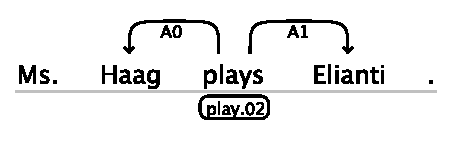
\includegraphics[scale=.63]{haag-example}
\end{center}
\end{quote}
we are to find out that for the predicate token {}``plays'' with sense ``play a 
role'' (play.02) the phrase headed by the token {}``Haag'' is referring to the 
player (A0) of the play event, and the phrase headed by the token {}``Elianti''  
is referring to the role (A1) being played. SRL is considered as a key task for 
applications that are required to answer questions such as {}``Who'', {}``What'', {}``Where'', etc.  

In this paper we introduce a Markov Logic~\citep[ML,][]{richardson06mln} approach to multi-lingual
SRL. We present a brief introduction to ML in 
section \ref{sec:markovlogic}.  At the core of ML are Markov Logic Networks~(MLN): sets of weighted First Order 
Logic (FOL) formulae. One attractive feature of the ML 
framework is that we can divide FOL formulae into subsets that serve as re-usable ``modules''. 
With this in mind we define MLN modules which capture the different stages of 
the task: argument identification, argument classification, and sense 
disambiguation. We also define modules for some of the language specific aspects of 
the task. We present all our ML modules in section 
\ref{sec:model}. These modules are the building blocks that we use to create 
MLNs for specific languages. We present our experiments and results for each of 
the languages of the task in section \ref{sec:results}.
% In section \ref{sec:analysis} we present some error analysis.



% we could wrap a supersection around the following 3 sections, but that 
% takes extra space. 

\section{IBM Model 4} 
\begin{eqnarray*}
 & p\left(a,f|e\right)=\\
 & \prod_{i=1}^{l}n\left(\phi_{i}|e_{i}\right)\times\prod_{i=1}^{l}\prod_{k=1}^{\phi_{i}}t\left(\tau_{ik},e_{i}\right)\times\\
 & \prod_{i=1,\phi_{i}>0}^{l}d_{1}\left(\pi_{i1}-c_{\rho_{i}}|class\left(e_{\rho_{i}}\right),class\left(\tau_{i1}\right)\right)\times\\
 & \prod_{i=1}^{l}\prod_{k=2}^{\phi_{i}}d_{>1}\left(\pi_{ik}-\pi_{i\left(k-1\right)}|class\left(\tau_{ik}\right)\right)\times\\
 & \left(\begin{array}{c}
m-\phi_{0}\\
\phi_{0}\end{array}\right)p_{1}^{\phi_{0}}\left(1-p_{1}\right)^{m-2\phi_{0}}\times\\
 & \prod_{k=1}^{\phi_{0}}t\left(\tau_{0k}|\text{NULL}\right)\end{eqnarray*}
 
 
\section{Integer Linear Programming Formulation}

\global\long\def\source{\mathbf{e}}
\global\long\def\target{\mathbf{f}}
\global\long\def\align{\mathbf{a}}
\global\long\def\start{\text{START}}
\global\long\def\stop{\text{END}}
\global\long\def\null{\text{NULL}}


Given a trained IBM model 4, and an input target sentence $\target$
we need to find the source sentence $\hat{\source}$ and alignment
$\hat{\align}$ with maximal $p\left(\align,\source|f\right)\backsimeq p\left(\source\right)\cdot p\left(\align,\target|\source\right)$.
{[}german at all etc{]} showed that we can formulate this problem
using Integer Linear Programming~{[}cite{]}. In this section we will
present our variant%
\footnote{Our formulation differs slightly because we use a first order modelling
language that imposed certain restrictions on the type of constraints
allowed.%
} of this ILP formulation. 

{[}German et al{]} framed the search for the highest scoring translation
(plus allignment) as the search for a single path over a set of source
candidate tokens $S$. Let $S_{i,10}$ be the 10 most likely translations
of $\target_{i}$ according to the probability $p\left(e|f_{i}\right)$.
Then $S$ is defined as

\[
S=\left\{ s_{I}^{e}|I\neq\emptyset\wedge\forall i\in I:e\in S_{i,10}\right\} \cup\left\{ s_{\left\{ \start\right\} },s_{\left\{ \stop\right\} }\right\} \]
That is, $S$ contains one token $s_{I}^{e}$ for each possible non-empty
set $I$ of target tokens that can likely generate the source word
$e$.%
\footnote{Note that this search space restriction is based on a reversal of
the noisy channel methaphor where source words generate target words.
This approach is consistent with previous work {[}German{]}, and signicantly
reduces the noise that would appear in a heuristic based on $p\left(f|e\right)$
instead. However, it should be remembered that strictly speaking we
(and {[}German{]}) do not perform optimal decoding in IBM Model 4,
but in a heuristically simplified version.%
} In addition, $S$ contains a $Start$ and an $End$ token to indicate
sentence beginning and end. For example, if a source word $is$ can
generate $f_{1}=CE$ and $f_{2}=NE$ of the sentence {}``CE NE EST
PAS CLAIR'', the $S$ contains, among others, $s_{\left\{ 1\right\} }^{is},s_{\left\{ 2\right\} }^{is}$
and $s_{\left\{ 1,2\right\} }^{is}$$ $. 

Each acyclic path $\left(s_{\left\{ \start\right\} },s_{1},\ldots,s_{n},s_{\left\{ \stop\right\} }\right)$
through $S$ that starts at $Start$ and ends at $End$ defines an
English sentence $\source$ by sequentially appending all non-Null
words $e$ of the $s_{I}^{e}$ tokens in the path. Such a path also
defines an alignment $\align$ as follows: a token $j=s_{I}^{e}$
that appears in a path is aligned to all tokens $i\in I$ of the target
sentence (in other words: source token $j=s_{I}^{e}$ generates all
target tokens in $I$).

We describe a path through the source tokens $S$ using two types
of variables. First, for each $s\in S$ we have a binary variable
$\alpha_{s}$ that indicates whether token $s$ is part of the path.
Second, we define a binary variable $\sigma_{s,t}$ for each $s_{I},t_{J}\in S$
with $I\cap J=\emptyset$ that indicates whether token $s$ is followed
by token $t$ in the source sentence. 
\begin{description}
\item [{Exactly~One~Source~Word}] For each target token $i$ there is
exactly one source token $s$ that generates it \[
\sum_{s_{I}^{e}|i\in I}\alpha_{s_{I}^{e}}=1\]

\item [{No~Cycles}] For all cycles $C\subseteq2^{S}$ of source words
\[
\sum_{\left(s_{1},s_{2}\right)\in C}\sigma_{s_{1},s_{2}}\leq1\]

\item [{Follows~Active~Consistency}] \[
\alpha_{s_{I}^{e}}=\sum_{s}\sigma_{s_{I}^{e},s}=\sum_{s}\sigma_{s,s_{I}^{e}}\]

\item [{Null~Target~Words}] We follow {[}German et. al{]} and require
that there is at most a single active$\null$ source token $s_{I}^{\null}$
, and that this token is not part of the actual path (or at its end).
We omit the corresponding constraints for brevity.
\end{description}
Finally, the linear objective function incorporates the model 4 probabilities
of a translation (as represented by an assignment for $f$ and $a$
variables) \[
\sum_{t}\sum_{s\in S\left(t\right)}w_{s}^{t}a_{s}^{t}+\sum_{s_{1},s_{2}}w_{s_{1},s_{2}}f_{s_{1},s_{2}}\]
 where $w_{s}^{t}$ is $\ldots$ and $w_{s_{1},s_{2}}$


\section{Cutting Plane Algorithm}
\global\long\def\y{\mathbf{y}}


The ILP program above has an exponential number of (cycle)
constraints. Hence, simply passing the ILP to an off-the-shelf ILP
solver is not practical for all but the smallest sentences. For this
reason \citet{GermannFast04} only consider sentences of up to eight
tokens. However, recent work~\citep{riedel06incremental} has shown
that even exponentially large decoding problems may be solved
efficiently using ILP solvers if a Cutting-Plane
Algorithm~\citep{dantzig54solution} is used.%
\footnote{It is worth mentioning that Cutting Plane Algorithms have
  been successfully applied for solving very large instances of the
  Travelling Salesman Problem, a problem essentially equivalent to the
  decoding in IBM Model 4.}

% In the following we will present a Cutting Plane algorithm for IBM
% Model 4:
% \begin{enumerate}
% \item Construct ILP $I$ without cycle constraints

% \begin{enumerate}
% \item \textbf{do}

% \begin{enumerate}
% \item solve $I$ and assign to solution $\y$
% \item find cyclic paths in solution $\y$
% \item add corresponding cycle constraints to $I$
% \end{enumerate}
% \textbf{until} no more cyclic paths can be found

% \item \textbf{return} $\y$
% \end{enumerate}
% \end{enumerate}
A Cutting-Plane Algorithm starts with a subset of the complete set of
constraints. In our case this subset contains all but the
(exponentially many) cycle constraints. The corresponding ILP is
solved by a standard ILP solver, and the solution is inspected for
cycles. If it contains no cycles, we have found the true optimum: the
solution with highest score that does not violate any constraints. If
the solution does contain cycles, the corresponding constraints are
added to the ILP which is in turn solved again. This process is
continued until no more cycles can be found.

% It is difficult to make claims about a guaranteed worst-case runtime
% (or number of iterations) of this algorithm. However, if the linear
% scoring function (in other words, the translation model and language
% model parameters) already provides a preference for cycle-free solutions,
% we can expect this algorithm to be efficient. For example, if we assume
% that the translation/distortion model has a very strong preference
% for monotonic solutions then clearly the highest scoring solution
% is likely to be cycle-free.




%%% Local Variables: 
%%% mode: latex
%%% TeX-master: "ilp-mt"
%%% End: 


\section{Results}

\section{Conclusion}


\end{document}
